%%%%%%%%%%%%%%%%%%%%%%%%%%%%%%%%%%%%%%%%%%%%%%%%%%%%%%%%%%%%%%%%%%%%%%%%%%%%%%%%
%%%%%%%%%%%%%%%%%%%%%%%%%%%%%%%%%%%%%%%%%%%%%%%%%%%%%%%%%%%%%%%%%%%%%%%%%%%%%%%%
%%%%%%%%%%%%%%%%%%%%%%%%%%%%%%%%%%%%%%%%%%%%%%%%%%%%%%%%%%%%%%%%%%%%%%%%%%%%%%%%
%%%%%%%%%%%%%%%%%%%%%%%%%%%%%%%%%%%%%%%%%%%%%%%%%%%%%%%%%%%%%%%%%%%%%%%%%%%%%%%%
\chapter{Systèmes du second ordre\label{annexe-2nd}}
%%%%%%%%%%%%%%%%%%%%%%%%%%%%%%%%%%%%%%%%%%%%%%%%%%%%%%%%%%%%%%%%%%%%%%%%%%%%%%%%
%%%%%%%%%%%%%%%%%%%%%%%%%%%%%%%%%%%%%%%%%%%%%%%%%%%%%%%%%%%%%%%%%%%%%%%%%%%%%%%%
%%%%%%%%%%%%%%%%%%%%%%%%%%%%%%%%%%%%%%%%%%%%%%%%%%%%%%%%%%%%%%%%%%%%%%%%%%%%%%%%
%%%%%%%%%%%%%%%%%%%%%%%%%%%%%%%%%%%%%%%%%%%%%%%%%%%%%%%%%%%%%%%%%%%%%%%%%%%%%%%%
Nous regroupons dans cette annexe les différents résultats obtenus lors de 
l'étude des système linéaires du second ordre. Ces ré
\newpage
%%%%%%%%%%%%%%%%%%%%%%%%%%%%%%%%%%%%%%%%%%%%%%%%%%%%%%%%%%%%%%%%%%%%%%%%%%%%%%%%
%%%%%%%%%%%%%%%%%%%%%%%%%%%%%%%%%%%%%%%%%%%%%%%%%%%%%%%%%%%%%%%%%%%%%%%%%%%%%%%%
%%%%%%%%%%%%%%%%%%%%%%%%%%%%%%%%%%%%%%%%%%%%%%%%%%%%%%%%%%%%%%%%%%%%%%%%%%%%%%%%
\section{Abaques de la réponse temporelle}
%%%%%%%%%%%%%%%%%%%%%%%%%%%%%%%%%%%%%%%%%%%%%%%%%%%%%%%%%%%%%%%%%%%%%%%%%%%%%%%%
%%%%%%%%%%%%%%%%%%%%%%%%%%%%%%%%%%%%%%%%%%%%%%%%%%%%%%%%%%%%%%%%%%%%%%%%%%%%%%%%
%%%%%%%%%%%%%%%%%%%%%%%%%%%%%%%%%%%%%%%%%%%%%%%%%%%%%%%%%%%%%%%%%%%%%%%%%%%%%%%%

%%%%%%%%%%%%%%%%%%%%%%%%%%%%%%%%%%%%%%%%%%%%%%%%%%%%%%%%%%%%%%%%%%%%%%%%%%%%%%%%
\paragraph{Dépassement}
%%%%%%%%%%%%%%%%%%%%%%%%%%%%%%%%%%%%%%%%%%%%%%%%%%%%%%%%%%%%%%%%%%%%%%%%%%%%%%%%
\begin{figure}[!h]
\begin{center}
        \tikzsetnextfilename{2nd_depassement_2-chap3-ext}
        \begin{tikzpicture}
    \pgfplotsset{signaltmp/.style={signaln,domain=0.0001:1,
                              unbounded coords=jump}
                }
    \pgfmathsetmacro{\pi}{3.141592653589793}     % dépassement d4 
    \begin{axis}
    [   xmode=log,
        ymode=log,
        width=0.65\textwidth,
        axis line style = thick,
        xmin=0.01,
        xmax=1,
        ymin=0.01,
        ymax=1.0,
        xlabel={$\xi$},
        ylabel={$D_k$},
        label style={font=\Large},
        grid=both,
        grid style={line width=.4pt, draw=black},
        major grid style={line width=.4pt,draw=black},
        legend style={draw=none,font=\normalsize},
        legend pos=outer north east,
        label style={font=\Large},
        legend cell align={left},
    ]
    \addplot[signaltmp,vtcol1] {exp(-(x*\pi)/(sqrt(1-x*x)))};
    \addplot[signaltmp,vtcol2] {exp(-(2*x*\pi)/(sqrt(1-x*x)))};
    \addplot[signaltmp,vtcol3] {exp(-(3*x*\pi)/(sqrt(1-x*x)))};
    \addplot[signaltmp,vtcol4] {exp(-(4*x*\pi)/(sqrt(1-x*x)))};
    \legend{$k=1$,$k=2$,$k=3$,$k=4$}
    \end{axis}
\end{tikzpicture}


\end{center}
\end{figure}

%%%%%%%%%%%%%%%%%%%%%%%%%%%%%%%%%%%%%%%%%%%%%%%%%%%%%%%%%%%%%%%%%%%%%%%%%%%%%%%%
\paragraph{Temps de réponse à 5\%}
%%%%%%%%%%%%%%%%%%%%%%%%%%%%%%%%%%%%%%%%%%%%%%%%%%%%%%%%%%%%%%%%%%%%%%%%%%%%%%%%
\begin{figure}
\centering
\tikzsetnextfilename{rapidite_tr_2ndordre-annexe-2nd-ext}
\begin{tikzpicture}
    \begin{axis}
    [   legend style={draw=none,font=\normalsize},
        legend pos=outer north east,
        axis line style = thick,
        width=0.75\textwidth,
        xmin=1e-1,
        xmax=1e1,
        ymin=1e0,
        ymax=1e2,
        xlabel={$\xi$},
        ylabel={$t_{5\%}\cdot\omega_0$},
        label style={font=\Large},
        legend cell align={left},
        xmode=log,
        ymode=log,
        grid=both,
        grid style={line width=.4pt, draw=black},
        major grid style={line width=.4pt,draw=black},
    ]%
        \addplot[mark=none,vtb,smooth]   table {python/tr.tab};
    \end{axis}
\end{tikzpicture}
\end{figure}

{\tikzset{external/export=false}
\begin{landscape}
    \newcommand{\mysize}{\footnotesize}
    \captionsetup{width=1.2\textwidth}
    \small
    \centering
    \captionof{table}{Formes caractéristiques des réponses temporelles d'un
                      système du second ordre pour les différents régimes.}
    \setlength{\ltmp}{0.25\textwidth}
    \setlength{\ldtmp}{0.34\textwidth}
    \ra{0.8}
    \begin{tabular}{@{}P{\ltmp}P{\ldtmp}P{\ldtmp}P{\ldtmp}@{}}%
    \toprule
    Réponse   & 
    Régime apérodique        ($\xi>1$)  & 
    Régime critique ($\xi=1$) & 
    Régime pseudo-périodique ($0<\xi<1$) \\
    \midrule
    Réponse impulsionnelle & 
    \raisebox{-.5\height}{\resizebox{\linewidth}{!}{\begin{tikzpicture}
    \begin{axis}
    [   legend style={draw=none},
        axis line style = thick,
        xmin=0,
        xmax=12,
        ymin=0,
        ymax=0.3,
        xlabel={$t$},
        ylabel={$s(t)$},
        label style={font=\Large},
        grid=both,
        grid style={line width=.4pt, draw=black},
        major grid style={line width=.4pt,draw=black},
    ]
    \addplot[signalb,domain=0:12] {(1/(3.73-0.26))*exp(-x/3.73)-exp(-x/0.26)};
    \end{axis}
\end{tikzpicture}
}} 
    $$
    s(t)=\dfrac{1}{\tau_1-\tau_2}
         \left(e^{-\frac{t}{\tau_1}}-e^{-\frac{t}{\tau_2}}\right)
    $$ &
    \raisebox{-.5\height}{\resizebox{\linewidth}{!}{    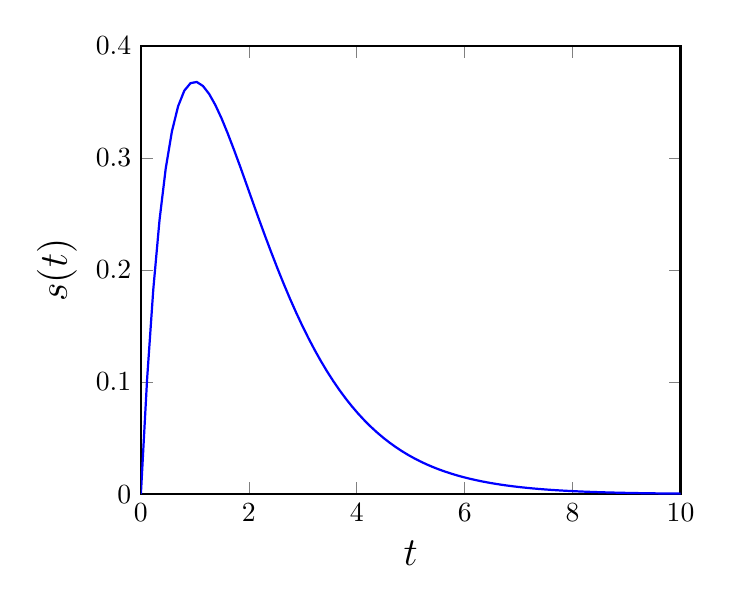
\begin{tikzpicture}
        \begin{axis}[
        legend style={draw=none},
        axis line style = thick,
        xmin=0,
        xmax=10,
        ymin=0,
        ymax=0.4,
        xlabel={$t$},
        ylabel={$s(t)$},
        label style={font=\Large},
        ]
            \addplot [thick,color=blue,domain=0:11.5, samples=101,unbounded coords=jump]{x*exp(-x)};
        \end{axis}
    \end{tikzpicture}
}} 
    $$
    s(t)=\dfrac{t}{\tau^2}e^{-\frac{t}{\tau}}
    $$ &  
    \raisebox{-.5\height}{\resizebox{\linewidth}{!}{\tikzsetnextfilename{2nd_rep_1_3_ext}
\begin{tikzpicture}
    \begin{axis}
    [   legend style={draw=none},
        axis line style = thick,
        xmin=0,
        xmax=12,
        ymin=-0.6,
        ymax=1.2,
        xlabel={$t$},
        ylabel={$s(t)$},
        label style={font=\Large},
        grid=both,
        grid style={line width=.4pt, draw=black},
        major grid style={line width=.4pt,draw=black},
    ]
    \def\a{0.3}            
    \def\b{0.91}           
    \def\w{0.953939201417} 
    \addplot[signalb,domain=0:12] {(\w/\b)*exp(-\a*x)*sin(deg(x)*\w)};
    \end{axis}
\end{tikzpicture}
}} 
    $$
    s(t)=\dfrac{\omega_d}{1-\xi^2}e^{-\xi\omega_0 t}\sin{\omega_d t}
    $$\\
    \midrule
    Réponse indicielle &  
    \raisebox{-.5\height}{\resizebox{\linewidth}{!}{\tikzsetnextfilename{2nd_rep_2_1_ext}
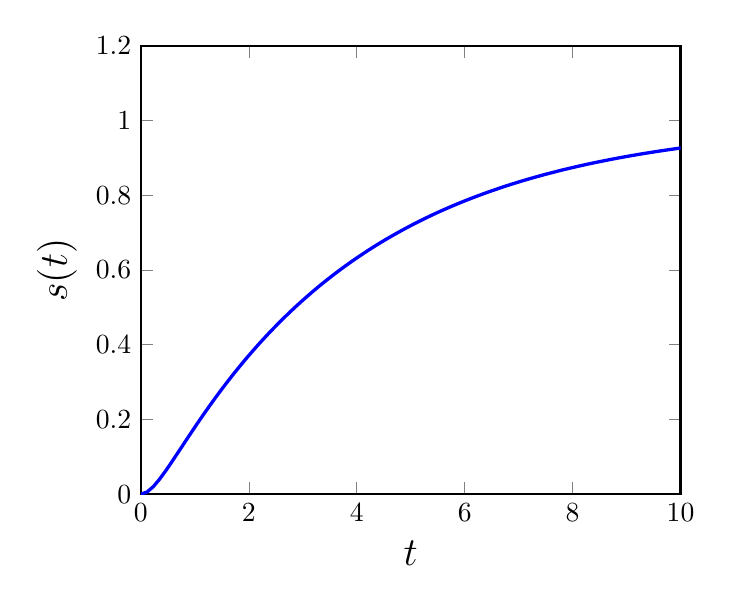
\begin{tikzpicture}
    \def\tu{2.0}
    \def\td{1.0}
    \begin{axis}
    [   legend style={draw=none},
        axis line style = thick,
        xmin=0,
        xmax=10,
        ymin=0,
        ymax=1.2,
        xlabel={$t$},
        ylabel={$s(t)$},
        label style={font=\Large},
    ]
    \addplot[very thick,color=blue,domain=0:11.5, samples=101]
    {1+(1/(3.73-0.26))*(0.26*exp(-x/0.26)-3.73*exp(-x/3.73))};
    \end{axis}
\end{tikzpicture}
}} 
    $$
    s(t)=1+\dfrac{1}{\tau_1-\tau_2}\left(\tau_2e^{-\frac{t}{\tau_2}}
                    -\tau_1e^{-\frac{t}{\tau_1}}\right)
    $$ &  
    \raisebox{-.5\height}{\resizebox{\linewidth}{!}{\begin{tikzpicture}
    \begin{axis}
    [   legend style={draw=none},
        axis line style = thick,
        xmin=0,
        xmax=10,
        ymin=0,
        ymax=1.2,
        xlabel={$t$},
        ylabel={$s(t)$},
        label style={font=\Large},
        grid=both,
        grid style={line width=.4pt, draw=black},
        major grid style={line width=.4pt,draw=black},
    ]
    \addplot[signalb,domain=0:10]  {1-exp(-x)-x*exp(-x)};
    \end{axis}
\end{tikzpicture}
}} 
    $$
    s(t)=1-e^{-\frac{t}{\tau}}-\dfrac{t}{\tau}e^{-\frac{t}{\tau}}
    $$ &  
    \raisebox{-.5\height}{\resizebox{\linewidth}{!}{\tikzsetnextfilename{2nd_rep_2_3_ext}
\begin{tikzpicture}
\begin{axis}
[   
    legend style={draw=none},
    axis line style = thick,
    xmin=0,
    xmax=12,
    ymin=0,
    ymax=1.5,
    xlabel={$t$},
    ylabel={$s(t)$},
    label style={font=\Large},
    grid=both,
    grid style={line width=.4pt, draw=black},
    major grid style={line width=.4pt,draw=black},
]
\def\a{0.3}            
\def\b{0.91}           
\def\w{0.954} 
\def\p{1.266}  
\addplot[signalb,domain=0:12] {1-((1./\w)*exp(-\a*x)*sin(deg(x)*\w+deg(\p)))};
\end{axis}
\end{tikzpicture}
}} 
    $$
    s(t) = 1 - \dfrac{e^{-\xi\omega_0 t}}{\sqrt{1-\xi^2}}\sin{(\omega_d t+\phi)}
    $$\\
    \bottomrule
    \end{tabular}
    \hspace{2em} 
    \begin{minipage}{18cm}
    \noindent
    \scriptsize
    \textbf{Paramètres : } (pour tous) $K=1$, $E_0=1$ (apériodique) 
    $\xi=2$, $\omega_0=1$ (i.e $\tau_1=3.73$ et $\tau_2=0.26$)
        (critique) $\xi=1$, $\omega_0=1$ (i.e $\tau=1$) (pseudo-périodique) $\xi=0.3$ et $\omega_0=1$
    \end{minipage}
\end{landscape}
\captionsetup{width=0.85\textwidth}

}
%\clearpage
%%%%%%%%%%%%%%%%%%%%%%%%%%%%%%%%%%%%%%%%%%%%%%%%%%%%%%%%%%%%%%%%%%%%%%%%%%%%%%%%
%%%%%%%%%%%%%%%%%%%%%%%%%%%%%%%%%%%%%%%%%%%%%%%%%%%%%%%%%%%%%%%%%%%%%%%%%%%%%%%%
%%%%%%%%%%%%%%%%%%%%%%%%%%%%%%%%%%%%%%%%%%%%%%%%%%%%%%%%%%%%%%%%%%%%%%%%%%%%%%%%
\section{Analyse fréquentielle}
%%%%%%%%%%%%%%%%%%%%%%%%%%%%%%%%%%%%%%%%%%%%%%%%%%%%%%%%%%%%%%%%%%%%%%%%%%%%%%%%
%%%%%%%%%%%%%%%%%%%%%%%%%%%%%%%%%%%%%%%%%%%%%%%%%%%%%%%%%%%%%%%%%%%%%%%%%%%%%%%%
%%%%%%%%%%%%%%%%%%%%%%%%%%%%%%%%%%%%%%%%%%%%%%%%%%%%%%%%%%%%%%%%%%%%%%%%%%%%%%%%

%%%%%%%%%%%%%%%%%%%%%%%%%%%%%%%%%%%%%%%%%%%%%%%%%%%%%%%%%%%%%%%%%%%%%%%%%%%%%%%%
\paragraph{Diagramme de Bode}
%%%%%%%%%%%%%%%%%%%%%%%%%%%%%%%%%%%%%%%%%%%%%%%%%%%%%%%%%%%%%%%%%%%%%%%%%%%%%%%%

\begin{figure}[!h]
\centering
\tikzsetnextfilename{bode_2nd_3-chap4-ext}
\newcommand{\LHS}[2][1.5em]{\hspace{#1}\mathllap{#2}}
\begin{tikzpicture}
\begin{axis}[
    name=ax1,
    ticklabel style = {font=\footnotesize},
    width=0.9\textwidth,
    height=0.25\textheight,
    ylabel={Gain (dB)},
    xtick={1e-1,1,1e1},
    ytick={-120,-100,-80,-60,-40,-20,0,20,40,60},
    xticklabels={$10^{-1}$,$10^{0}$,$10^{1}$},
    yticklabels={-120,-100,-80,-60,-40,-20,0,20,40,60},
    xmode=log,ymode=normal,
    xmin=1e-1, xmax=1e1,
    ymin=-40, ymax=30,
    grid=both,
    major grid style={black!40},
    cycle list name=fmvcolist,
]
    \foreach \a in {0.02,0.1,0.2,0.3,0.4,0.5,0.6}
    \addplot+[very thick,domain=1e-1:1e1, samples=201] 
    {-20*log10(sqrt((1-x*x)^2+(2*\a*x)^2))};
\end{axis}
\begin{axis}[
    at={(ax1.south west)},
    yshift=-12em,
%    xshift=-14em,
    legend style={draw=none,yshift=1em},
    legend pos=outer north east,
    ticklabel style = {font=\footnotesize},
    width=0.9\textwidth,
    height=0.25\textheight,
    xlabel={Pulsation (rad/s)},
    ylabel={Phase (degré)},
    xtick={1e-1,1,1e1},
    ytick={-180,-135,-90,-45,0},
    yticklabels={-180,-135,-90,-45,0},
    xticklabels={$10^{-1}$,$10^{0}$,$10^{1}$},
    xmode=log,ymode=normal,
    xmin=1e-1, xmax=1e1,
    ymin=-180, ymax=0,
    grid=both,
    major grid style={black!40},
    cycle list name=fmvcolist,
]
    \foreach \a in {0.02,0.1,0.2,0.3,0.4,0.5,0.6}
    \addplot+[very thick,domain=1e-1:1e1, samples=201] {-atan2(2*\a*x,(1-x*x))};

    \legend{$\LHS{\xi}=0.02$,$\LHS{\xi}=0.1$,$\LHS{\xi}=0.2$, 
            $\LHS{\xi}=0.3$, $\LHS{\xi}=0.4$,$\LHS{\xi}=0.5$, 
            $\LHS{\xi}=0.6$, $\LHS{\xi}=0.7$, $\LHS{\xi}=0.8$, $\LHS{\xi}=0.9$}
\end{axis}
\end{tikzpicture}


%\caption{Diagramme de Bode d'une fonction de transfert du 2nd ordre 
%(\Cref{eq-2nd_ftjw}) pour
%différentes valeurs de $\xi$ avec $K=1$ et $\omega_0=1$\label{fig-bode_1er_2}}
\end{figure}

%%%%%%%%%%%%%%%%%%%%%%%%%%%%%%%%%%%%%%%%%%%%%%%%%%%%%%%%%%%%%%%%%%%%%%%%%%%%%%%%
\paragraph{Phénomène de résonance}
%%%%%%%%%%%%%%%%%%%%%%%%%%%%%%%%%%%%%%%%%%%%%%%%%%%%%%%%%%%%%%%%%%%%%%%%%%%%%%%%

\begin{figure}[!h]
    \centering
    \tikzsetnextfilename{gain_resonance-chap4-ext}
    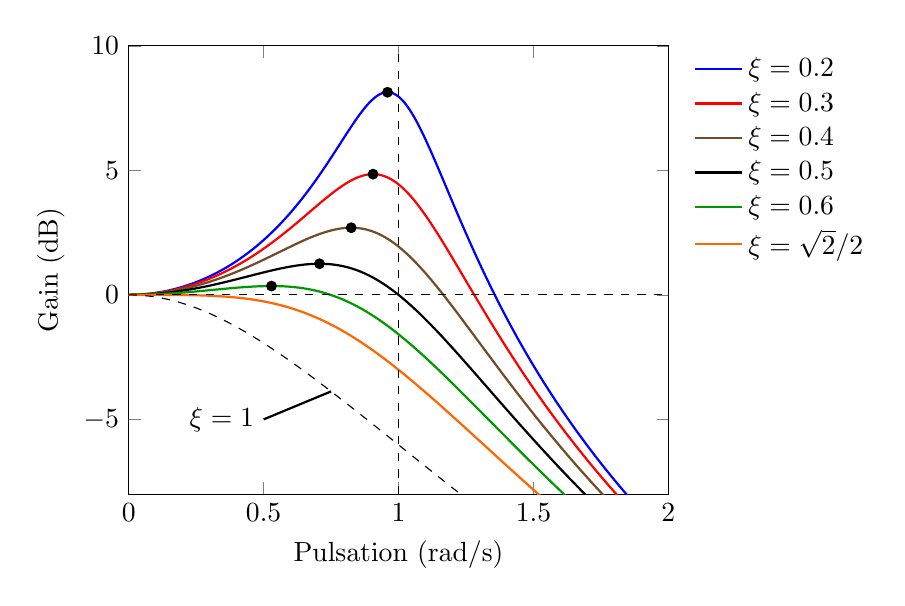
\begin{tikzpicture}
    \pgfplotscreateplotcyclelist{mycolorlist}{%
            blue\\%
            red\\%
            brown!60!black\\%
            black\\%
            green!60!black\\%
            red!60!yellow\\
            }
    \begin{axis}
    [   ticklabel style = {font=\normalsize},
        legend style={draw=none},
        legend pos=outer north east,
        legend cell align={left},
        ylabel={Gain (dB)},
        xlabel={Pulsation (rad/s)},
        xmode=normal,ymode=normal,
        xmin=0.0, xmax=2,
        ymin=-8, ymax=10,
        major grid style={black!40},
        cycle list name=mycolorlist,
    ]
    \foreach \a in {0.2,0.3,0.4,0.5,0.6,0.707} 
    \addplot+[thick,domain=0:2,samples=201] 
    {-20*log10(sqrt((1-x*x)^2 +(2*\a*x)^2))};

    \addplot[dashed,domain=0.1:5,samples=201] {0};
    \def\a{1.0}
    \addplot[dashed,domain=0:2,samples=201] 
    {-20*log10(sqrt((1-x*x)^2 +(2*\a*x)^2))};
    \coordinate (P) at 
    (axis cs:0.75,{-20*log10(sqrt((1-0.75*0.75)^2 +(2*\a*0.75)^2 ))});
    \node[left] (a) at (axis cs:0.5,-5) {$\xi=1$};
    \draw [thick] (a.east) -- (P);
    \addplot[mark size=1.75pt,black,fill=black,mark=*,only marks] 
    coordinates {
            (0.959166304663,8.13608784305)
            (0.905538513814,4.84656106912)
            (0.824621125124,2.69540739954)
            (0.707106781187,1.24938736608)
            (0.529150262213,0.354575339209)
    };
    \draw[dashed] (axis cs:1,-10) -- (axis cs:1,10);
    \legend{$\xi=0.2$,$\xi=0.3$,$\xi=0.4$,$\xi=0.5$,$\xi=0.6$,$\xi=\sqrt{2}/2$}
    \end{axis}
\end{tikzpicture}


%\caption{\'Evolution du gain en décibel en fonction de la pulsation pour 
%différentes valeur du taux d'amortissement du régime pseudo-périodique. 
%Le gain maximal à la pulsation de résonance $\omega_r$ est représenté par 
%une pastille noir sur chacune des courbes pour $\xi<\sqrt{2}/2$. 
%On remarquera l'utilisation exceptionnel 
%d'une échelle linéaire pour les pulsations.}
\end{figure}
%%%%%%%%%%%%%%%%%%%%%%%%%%%%%%%%%%%%%%%%%%%%%%%%%%%%%%%%%%%%%%%%%%%%%%%%%%%%%%%%
%%%%%%%%%%%%%%%%%%%%%%%%%%%%%%%%%%%%%%%%%%%%%%%%%%%%%%%%%%%%%%%%%%%%%%%%%%%%%%%%
%%%%%%%%%%%%%%%%%%%%%%%%%%%%%%%%%%%%%%%%%%%%%%%%%%%%%%%%%%%%%%%%%%%%%%%%%%%%%%%%
%%%%%%%%%%%%%%%%%%%%%%%%%%%%%%%%%%%%%%%%%%%%%%%%%%%%%%%%%%%%%%%%%%%%%%%%%%%%%%%%
%annexe_2nd.tex
